\section{Theoretical Background}\label{theoreticalBackground}


\subsection{Formal Languages and Formal Grammars}\label{formalLanguages}
A formal language $L$ is defined as a subset of $\Sigma^{*}$ over an alphabet $\Sigma$, with $\Sigma^{*}$ being the set of all words over the alphabet. For the purpose of formal language theory, the subset of $\Sigma^{*}$ that constitutes the language $L(G)$ needs to be well-formed given the formal grammar $G$.
As per \cite{JurafskyMartin2009}, the definition of a formal grammar is $G = \lbrace N, \Sigma, R, S \rbrace$, where $N$ is a set of non-terminal symbols, $\Sigma$ is a set of terminal symbols (alphabet), $R$ is a set of rules of the form $\alpha \rightarrow \beta$ (where $\alpha$ and $\beta$ are strings of symbols from $(\Sigma \cup N)^{*}$) and $S$ is a designated start symbol.

$L(G)$ consists of all strings $w$ that can be derived from the start symbol $S$ in a finite number of steps, formally $\lbrace w \in \Sigma^{*} | S \xRightarrow [\text{G}]{\text{*}} w \rbrace$. As such, a word $w \in \Sigma^{*}$ that cannot be derived from $S$ in a finite number of steps is not part of $L(G)$.

Formal grammars differ in terms of complexity and can be described in a hierarchical manner. Grammars of higher complexity have a greater generative power than grammars of lower complexity. The most commonly used hierarchy of grammars is the Chomsky hierarchy (\cite{Chomsky1959}). In this hierarchy, formal grammars are classified into three types, sorted from most powerful to least powerful: Turing equivalent (Type 0), Context Sensitive (Type 1), Context Free (Type 2) and Regular (Type 3).

The difference in generative power and complexity stems from increasing restrictions imposed on the rules of the grammar - a Type 3 grammar is more restrictive than a Type 0 grammar. As such, every grammar of a higher type is a subset of the previous type of grammar. A visual representation of this property can be found in Figure \ref{fig:ChomskyHierarchy}.

\begin{figure}[htb]
 \centering
 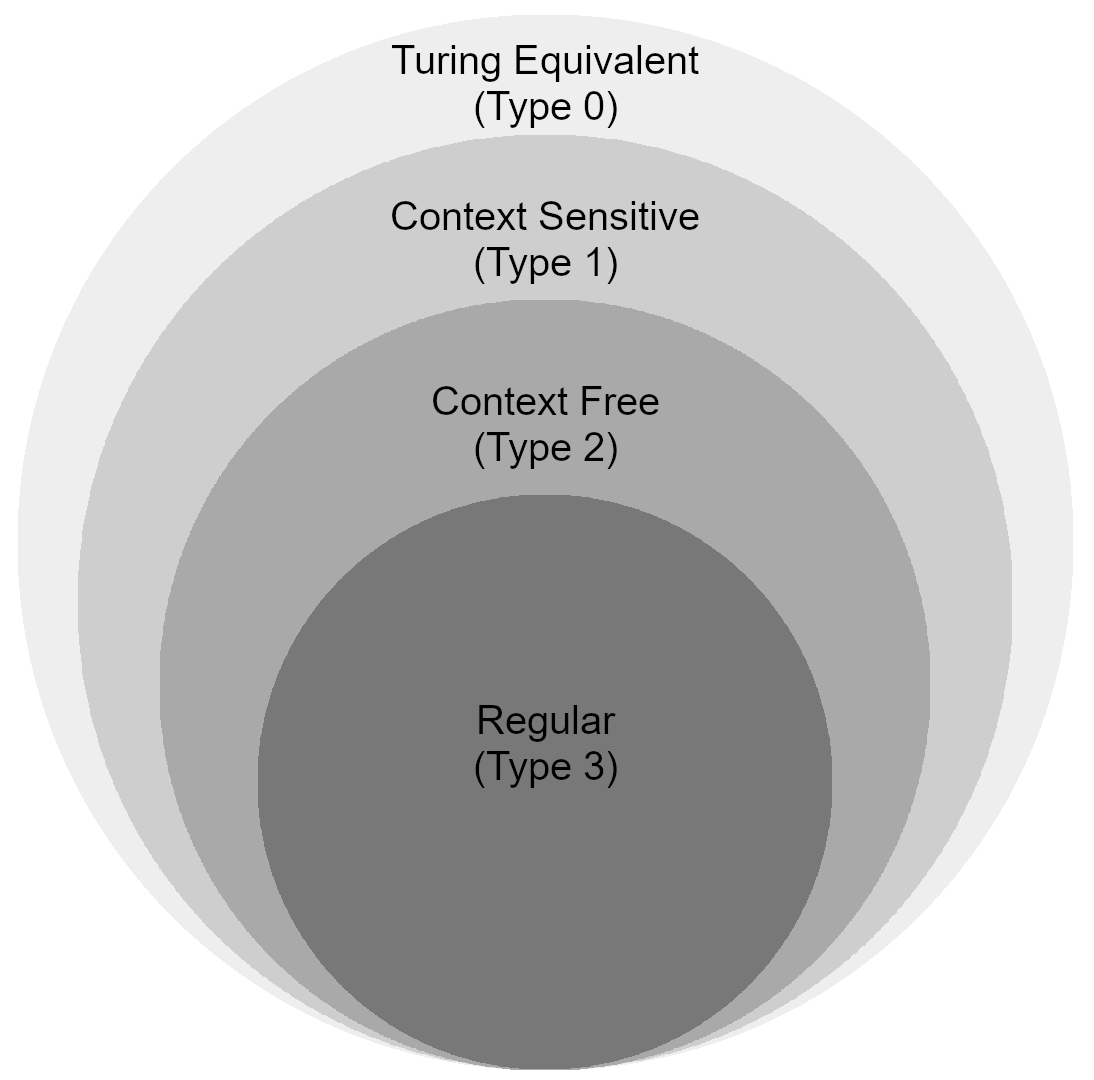
\includegraphics[width=0.5\linewidth]{abb/chomskyhierarchy}
 \caption[Chomsky Hierarchy]{A visual representation of the Chomsky Hierarchy.}
\label{fig:ChomskyHierarchy}
\end{figure}

The four types of formal grammars can be defined by the form their rules can take. An overview over these rules as per \cite{JurafskyMartin2009} can be found in Table \ref{tab:GrammarRules}, where $A$ is a single non-terminal, $\alpha$, $\beta$, $\gamma$ are strings of terminal and non-terminal symbols, and $x$ is a string of terminal symbols. $\alpha$, $\beta$ and $\gamma$ may be empty unless specifically disallowed. The table is supplemented with a column describing the corresponding automaton capable of accepting or recognizing the grammar.

\begin{table}[b]
	\begin{tabularx}{\textwidth}{@{}l*{10}{C}c@{}}
	\toprule 
	\textit{Type} & \textit{Name} & \textit{Rule Skeleton} & \textit{Automaton}\\ 
	\toprule	
	0 & Turing Equivalent & $\alpha \rightarrow \beta$, s.t. $\alpha \neq \epsilon$ & Turing Machine (recognized) \\
	1 & Context Sensitive & $\alpha A \beta \rightarrow \alpha \gamma \beta$, s.t. $\gamma \neq \epsilon$ &  Linear Bound Automata (accepted) \\
	2 & Context Free & $A \rightarrow \gamma$ & Push Down Automata (accepted) \\
	3 & Regular & $A \rightarrow xB$ or $A \rightarrow x$ & Finite-State Automata (accepted) \\
	\bottomrule	
	\end{tabularx}
	\caption[Overview of formal grammar properties.]{Overview of formal grammar properties according to \cite{JurafskyMartin2009}, augmented with corresponding automata.}
	\label{tab:GrammarRules}
\end{table}

\subsection{Formal Grammars and Natural Language}
The correspondence of formal grammars to automata and Computational Complexity Theory lends itself to consider natural languages under the same lense. While formal grammars constitute powerful tools with which phenomena in natural language can be described, assessing precisely where natural languages lie within the Chomsky hierarchy is the subject of ongoing research.
The usual form arguments answering that question take is one of finding lower bounds: If there is a phenomenon in a natural language that cannot be described with a given grammar, natural language must be - however slighty - more complex than that type allows. Such arguments increase in credibility the more frequently they can be replicated for phenomena in multiple languages. The arguments establishing natural languages as supra-context-free (i.e. more complex than CFGs) as well as contrary evidence from empiric research shall be presented here.

\subsubsection{Natural Language as supra-regular}\label{supraReg}
English, as well as several other languages (\cite{Hagege1976}) allow for center embedding, the embedding of a phrase into another phrase of the same type.
%\begin{exe}
%	\ex The man eats.
%	\ex The man the boss fired eats.
%	\ex The man the boss the investor distrusted fired eats.
%	\ex The man the boss the investor the police investigated distrusted fired eats.
%\end{exe}
Let the set $E$ contain all grammatical sentences of English, and let the noun phrases and transitive verbs constitute following sets:
\begin{align*}
A &= \lbrace \text{the boss}, \, \text{the investors}, \, \text{the police}, \dots \rbrace \\
B &= \lbrace \text{fired}, \, \text{distrusted}, \, \text{investigated}, \dots \rbrace
\end{align*}
Then the following two sets can be defined.
\begin{align*}
E' &= \lbrace \text{the man } a^{n}b^{n} \text{ eats} \: \vert \: n \geq 0 \rbrace \\
R &= \lbrace \text{the man } a^{*}b^{*} \text{ eats} \rbrace
\end{align*}
$a^{n}$ and $b^{n}$ are finite sequences of size $n$ of elements of sets $A$ and $B$, respectively. $E'$ describes a subset of $E$, namely $E \cap R$. Since regular languages are closed under intersection and $E'$ is not regular, $E$ is not regular.\footnote{The proofs for regular languages being closed under intersection and $E'$ not being regular can be found in the appendix.}

While this proof is correct under the framework of Formal Language Theory, the validity of claiming that it shows natural language to be supra-regular is debatable. Research in psycholinguistics shows that native speakers have face severe problems processing center embeddings of depth two or higher, yielding long processing times, an incomplete understanding of the presented sentence or leading the participants to judge the sentence as ungrammatical (\cite{Hamilton1971}, \cite{Frank2016}). Furthermore, the corpus-driven analysis by \cite{Karlsson2007} suggests an upper limit of center embedding depth three in the seven investigated languages.

The proof concerns linguistic competence, whereas empirical studies provide an insight into linguistic performance. Usually, the distinction between competence and performance provide an adequate framework for both theoretical and empirical work, but when discussing the complexity of natural language neither side should be discarded. A linguistic competence framework cannot appropriately declare natural language as supra-regular if natural language is produced and processed according to regular rules. Conversely, for the purposes of computational linguistics, exclusively assessing linguistic performance by way of corpus analysis is insufficient, as a corpus of any size pales in comparison to the potential for infinitely many combinations that characterizes language. For the purposes of NLP, it is recommendable to err on the side of overestimating the complexity of natural language - so long as the resulting models are sufficiently efficient and accurate.

\subsubsection{Natural Language as supra-context-free}

Similarly to the proof given in Section \ref{supraReg}, an argument characterizing natural language as supra-context-free can be brought forth. It is based on embedded infinitival verb phrases found in Swiss German (\cite{Shieber1987}).
%\begin{exe}
%	\ex
%	\gll Jan säit das mer em Hans es huus haend wele hälfe aastriiche. \\
%	Jan said that we the Hans-DAT the house-ACC have wanted help paint \\
%	\trans 'Jan said that we have wanted to help Hans paint the house.'
%	\ex
%	\gll Jan säit das mer d'chind em Hans es huus haend wele laa hälfe aastriiche. \\
%	Jan said that we the children-ACC the Hans-DAT the house-ACC have wanted let help paint \\
%	\trans 'Jan said that we have wanted to let the children help Hans paint the house.'
%\end{exe}

Four finite sets can be constructed from these examples: accusative noun phrases ($A = \lbrace \text{d'chind}, \, \dots \rbrace$), dative noun phrases ($B = \lbrace \text{em Hans}, \, \dots \rbrace$), transitive verbs taking accusative objects ($C = \lbrace \text{laa}, \, \dots \rbrace$) and transitive verbs taking dative objects ($D = \lbrace \text{hälfe}, \, \dots \rbrace$). Let the set $S$ then be the set of all grammatical sentences of Swiss German. Again, the two following sets can be defined:
\begin{align*}
S' &= \lbrace \text{Jan säit das mer } a^{n}b^{m} \text{ es huus haend wele } c^{n}d^{m} \text{ aastriiche} \: \vert \: n, m \geq 0 \rbrace \\
R &= \lbrace \text{Jan säit das mer } a^{*}b^{*} \text{ es huus haend wele } c^{*}d^{*} \text{ aastriiche} \rbrace
\end{align*}
$S'$ is not context-free and results from $S \cap R$. Since context-free sets are closed under intersection with regular sets, $G$ cannot be not context-free.\footnote{The respective proofs for $S'$ not being context-free and context-free sets being closed under intersection with regular sets can be found in the Appendix.}

Curiously enough, empirical research into the matter of processing similar cross-serial dependencies in Dutch suggests them to be generally easier to process than nested dependencies (i.e. the ones used to prove natural language to be supra-regular) (\cite{Bach1986}).

\subsection{Dyck Languages}\label{dyckLanguages}
Whether natural language is regular, context-free, supra-regular or supra-context-free is a distinction of only tangential relevance for this work. The first two cases are fully covered by CFGs, while the other two leave room for some natural language productions outside of the scope of CFGs. The characteristics of supra-context-free examples in natural language show a \textit{weak} non-context-freeness, making CFGs sufficient for covering the vast majority of natural language productions. With this assumption, an appropriate CFG for a model to learn must be found. The most important property of this grammar is that model performance on its language must allow for strong conclusions about the learnability of any other CFG. In doing so, one can make reasoned assumptions about potential model performance on natural language data. 

One such a grammar is the Dyck Grammar, which can produce an array of Dyck Languages. Let $D_{n} = \lbrace N, \Sigma, R, S \rbrace$ with
\begin{align*}
	N &= \lbrace S \rbrace \\
	\Sigma &= \lbrace \epsilon, O_{1}, O_{2}, \dots, O_{n}, C_{1}, C_{2}, \dots, C_{n} \rbrace \\
	R &= \lbrace \\
		 & \: S \rightarrow \epsilon \\
		 & \: S \rightarrow O_{n} \, S \, C_{n} \, \rbrace ,
\end{align*}
where $O_{n}$ represents an opening parenthesis, $C_{n}$ represents a closing parenthesis and $n$ denotes the number of distinct pairs of parentheses. $D_1$, then, denotes the Dyck Language with $\Sigma = \lbrace \epsilon, (, ) \rbrace$, $D_2$ the Dyck Language with $\Sigma = \lbrace \epsilon, (, [, ], ) \rbrace$, et cetera.

Within the family of Dyck Languages, $D_2$ is of particular interest. According to the Chomsky-Schützenberger Representation Theorem \citep{Chomsky1963}, for every context-free language $L$ there exists a positive integer $n$, a regular language $R$, and a homomorphism $h$ so that $L = h(D_{n} \cap R)$. Following the proof in \cite{Autebert1997}, a homomorphism $g_{n}$ can be constructed so that $D_{n} = g_{n}^{-1}(D_{2})$. It follows that every context-free language can be represented as $L = h(g_{n}^{-1}(D_{2}) \cap R)$. As such, every CFL could be represented via homomorphisms on $D_2$ and intersections with a regular language\footnote{NDFL vs DFL!}. Assuming natural languages to be context-free and bearing in mind that using a formal language is a choice of abstraction which allows for precise control over corpus composition, this makes $D_2$ the language of choice when evaluating neural network performance on a comparative scale.
%TODO proof, basically
%TODO NDFL vs DFL footnote

\subsection{Neural Network Architectures}\label{neuralNetworkArchitectures}

\subsubsection{Simple RNN}\label{SRNN}
Recurrent Neural Networks (RNNs) (\cite{Elman1990}) are a neural network architecture particularly suited to processing sequential information by virtue of them being recurrent: the RNN's output at a time step $t$ is fed back as its input at the following time step $t+1$. As such, every output is dependent on the previous computation as well as the current input. This property equips RNNs with a "memory" with regards to previous inputs, allowing them to capture context dependencies a context agnostic model cannot adequately learn.

Within the frame of this work, the specific case of the Simple RNN (SRNN) is considered. It is a three layer networks, consisting of an input layer, a hidden layer and an output layer. The hidden state $h_t$ at time step $t$ given the input vector $x_t$ and the output vector $y_t$ are calculated as per the following equations:

\begin{align}
	h_{t} &= f(\boldsymbol{W_{xh}} x_{t} + \boldsymbol{W_{hh}} h_{t-1}) \\
	y_{t} &= \boldsymbol{W_{hy}} h_{t}
\end{align}

The function $f$ constitutes a non-linear transformation, like $\tanh$ or ReLU. $\boldsymbol{W_{xh}}$, $\boldsymbol{W_{hh}}$, $\boldsymbol{W_{yh}}$ are matrices of the weights connecting the input layer to the hidden layer, the hidden layer to itself and the hidden layer to the output layer, respectively.

When training RNNs, it is beneficial to think of the network as unfolding into an architecture with one layer per time step. A visualisation is provided in Figure \ref{fig:unrolledRNN}. As such, the RNN can be treated as a deep feedforward network. These conceptual layers share their parameters - if any weight changes at time step $t$, the weight also changes at $t+1, t+2, \dots, t+n$. Isolated changes are not possible. A popular training algorithm for RNNs is Backpropagation Through Time (BPTT) (\cite{Williams1998}), a gradient based algorithm designed for recurrent rather than feedforward networks. However, as \cite{Bengio1994} and \cite{Hochreiter1998} show, RNNs suffer from a fundamental flaw: the aptly named vanishing gradient problem, in which the training gradient diminishes to zero throughout the layers.

\begin{figure}[htb]
 \centering
 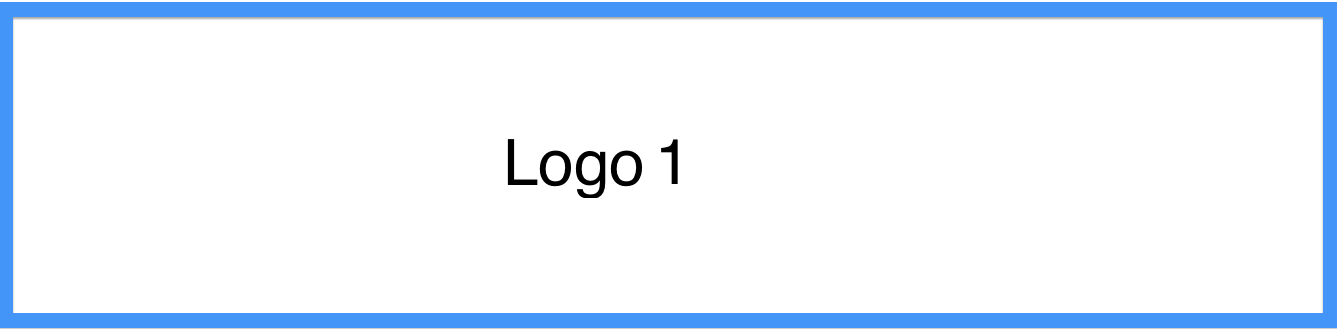
\includegraphics[width=0.6\textwidth]{abb/logo1}
 \caption[Unfolded RNN]{An RNN, unfolded through time.}
\label{fig:unrolledRNN}
\end{figure}

%TODO RNN unfold graphic (check Young et al. 2018 p.11 for an example
%TODO (maybe!) brief overview of sources utilizing RNNs for NLP and formal language eval

\subsubsection{LSTM}\label{LSTM}

Long-Short Term Memory networks (LSTM) were designed by \cite{Hochreiter1997} as an RNN architecture which preserves the RNN capabilities of processing sequential data of arbitrary length and capturing context dependencies, while circumventing the vanishing gradient problem.

LSTMs are based on self-connected linear units which are regulated by three multiplicative gates: input (in), output (out) and forget ($\varphi$). At every time step, the concatenated vector of the previous hidden state $h_{t-1}$ and the current input $x_{t}$ are received by all three gates. Given this input, the gates apply individual multiplicative factors $m_{\text{Gate}} \in [0, \dots, 1]$, determining what information is let through the input gate, passed through the output gate or forgotten by the self-connected linear unit.

\begin{align*}
\text{in}_{t} &= m_{\text{in}} (\boldsymbol{W_{\text{in}}} \cdot [h_{t-1},x_{t}] + b_{\text{in}}) \\
\text{out}_{t} &= m_{\text{out}} (\boldsymbol{W_{\text{out}}} \cdot [h_{t-1},x_{t}] + b_{\text{out}}) \\
\varphi_{t} &= m_{\varphi} (\boldsymbol{W_{\varphi}} \cdot [h_{t-1},x_{t}] + b_{\varphi})
\end{align*}

Finally, the cell state $C_{t-1}$ is updated to $C_{t}$ and $h_{t}$ is set.

\begin{align*}
C_{t} &= \text{forget}_{t} \odot C_{t-1} + \text{in}_{t} \odot \tanh (\boldsymbol{W_{C}} \cdot [h_{t-1},x_{t}] + b_{\text{C}}) \\
h_{t} &= \text{out}_{t} \odot \tanh (C_{t})
\end{align*}

\begin{figure}[htb]
 \centering
 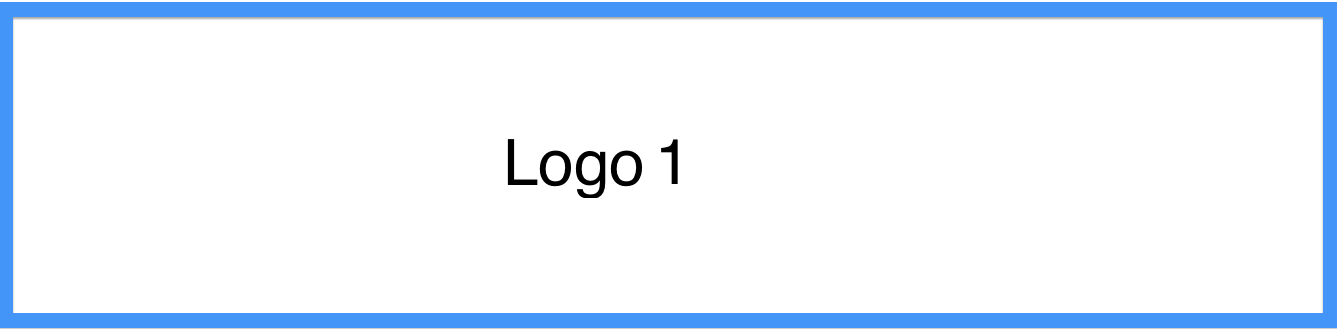
\includegraphics[width=0.6\textwidth]{abb/logo1}
 \caption[LSTM Memory Cell]{An LSTM memory cell, bla, bla bla.}
\label{fig:memoryCellLSTM}
\end{figure}

%TODO LSTM memory cell figure (check Hochreiter 1997 or explanations for reference)
%TODO (maybe!) brief overview of sources utilizing LSTMs for NLP and formal language eval

\subsubsection{GRU}\label{GRU}
A less complex alternative to LSTMs, the Gated Recurrent Unit (GRU) was developed by \cite{Cho2014}. The information flow within the GRU is handled by just two gates: reset ($r$) and update ($z$). The update gate determines how much information from previous time steps is passed along for further time steps, while the reset gate enables the model to drop irrelevant information and only consider the current input rather than the previous hidden state, as described in the equations below, where $j$ is the $j$-th hidden unit, $\sigma$ is the squashing sigmoid function, $\boldsymbol{W}$ and $\boldsymbol{U}$ are learned gate-dependent weight matrices and $\phi$ is a non-linear function.

\begin{align*}
r_j &= \sigma \big( [\boldsymbol{W_{r}}x]_{j} + [\boldsymbol{U_{r}}h_{t-1}]_{j} \big) \\
z_j &= \sigma \big( [\boldsymbol{W_{z}}x]_{j} + [\boldsymbol{U_{z}}h_{t-1}]_{j} \big) \\
h_{j}^{t} &= z_{j}h_{j}^{t-1} + (1 - z_{j}) \tilde{h}_{j}^{t} \\
\tilde{h}_{j}^{t} &= \phi \big( [\boldsymbol{W}x]_{j} +[\boldsymbol{U}(r \odot h_{t-1}]_{j}) \big)
\end{align*}

\begin{figure}[htb]
 \centering
 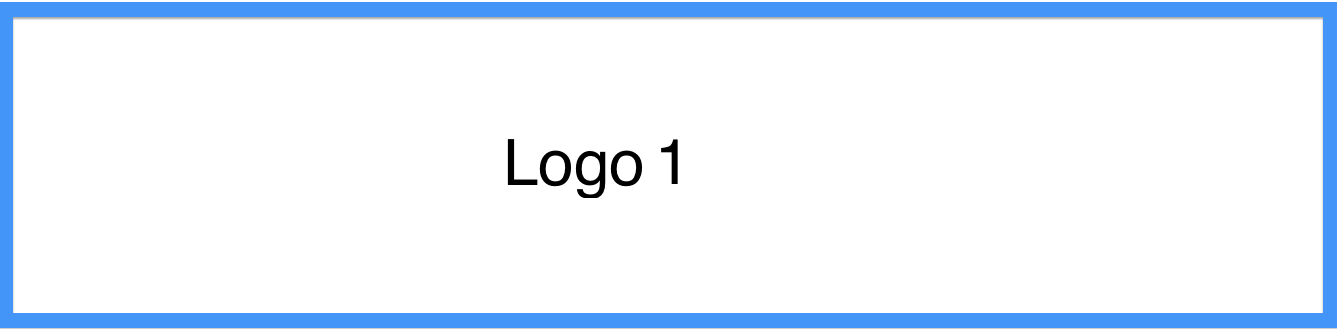
\includegraphics[width=0.6\textwidth]{abb/logo1}
 \caption[Illustration of a GRU]{Illustration of a GRU.}
\label{fig:GRU}
\end{figure}

%TODO GRU figure (see Young et al. 2018 page 12/Cho et al 2014 for reference)
%TODO (maybe!) brief overview of sources utilizing GRUs for NLP and formal language eval

\subsection{Related Works}\label{relatedWorks}

Formal languages have been used to evaluate the performance of neural network architectures for decades (\cite{Cleeremans1989}, \cite{Zeng1994}, \cite{Hochreiter1997}, \cite{Rodriguez1998}, \cite{GersSchmidhuber2001}, \cite{JoulinMikolov2015}). These papers frequently determine how well the architecture can generalize from training on a relatively small subset of the language to testing on longer unseen words. (Example results)
%TODO Specific example results, i.e. "LSTMs can learn CSLs"
%TODO include research into automaton extraction from neural networks for regular and context-free grammars


While these results make for compelling cases in favour of the architectures proposed by the authors, the methodology has recently come under criticism by researchers like \cite{Bernardy2018}, \cite{Sennhauser2018}. The former goes as far as to say that none of the previous research compellingly shows RNNs to be capable of learning nested hierarchical structures.
%TODO Reread and specifically state Bernardy's criticism


Formal languages making up early performance benchmarks for neural networks was, in the early years of RNN research, at least partially caused by the lack of comparable natural language corpora and of reliable hardware with sufficient computational power. By now, of course, these restrictions are far above the levels of 1990 (Elman RNN). This lead to a sizeable corpus of research on NLP, i.e. \cite{Karpathy2015}.
%TODO more elegant mention of NLP research and NLP application


There are several recent works investigating neural architectures and their capability of learning Dyck languages specifically. [They feature a variety of ways of sampling their corpora, evaluate models on different tasks and report a varying subset of relevant performance measures.]

\cite{Deleu2016} evaluate the capability of a Neural Turing Machine (NTM) to deal with long-term dependencies. The model performs a membership classification task on words belonging to D$_1$ and non-words using the same alphabet, but not belonging to D$_1$. The NTM shows strong generalization by correctly recognizing well over $90 \%$ of D$_1$ words with length 180, despite only being trained on words of length $<12$. The authors do not report on any other measures of performance.

\cite{Li2018} deserve a mention in this section for evaluating their nonlinear weighted finite automata on a corpus generated by a probabilistic D$_1$ grammar and reporting on word error rate (WER) relative to the size of the training set. The size of the training set ranges from $200$ to $20,000$, with a fixed test set size of $250$.

\cite{Skachkova2018} compare the accuracy and perplexity of Elman-RNNs, GRUs and LSTMs learning D$_1$, D$_2$, D$_3$, D$_4$ and D$_5$. The respective corpora are generated by a probabilistic Dyck grammar, with the given rule probabilities controlling the average length of the generated sequences.

\cite{Sennhauser2018} choose an approach that demonstrates whether an LSTM can learn hierarchical structures by training the models for a prediction task on one million D$_2$ words with length 100. Their training corpus has been sampled from a probabilistic D$_2$ grammar. They report on two further corpus properties: distance, which is the number of characters between an opening bracket and its corresponding closing bracket, and embedded depth, which is the maximum number of unclosed brackets in a processed word. They report error rate, predictable distances and embedded depth in relation to number of hidden units. Furthermore, they perform an Intermediate State Analysis. Their results suggest the trained models fail at correctly learning the rules of the D$_2$ grammar.

\cite{Suzgun2019} offer an overview of small-sized Elman-RNNs, GRUs and LSTMs learning D$_1$, D$_2$ and corresponding shuffle languages. They report accuracy and provide an analysis of the LSTM cell state dynamics. They find that none of their models are capable of learning D$_2$, with the highest scoring model (LSTM) achieving a $48.24\%$ accuracy.

The topic of investigation of \cite{Yu2019} lies outside of the scope of this thesis, as it is predominantly concerned with the seq2seq framework and attention mechanisms. However, their data set consists of largely the same settings as \cite{Sennhauser2018} have used. Additionally, they report many of the same measures of performance.

An overview of investigated Dyck languages, corpus sizes and reported measures of performance can be found in Tables \ref{tab:LiteratureCorpusOverview}, \ref{tab:LiteratureInvestigatedModels} and \ref{tab:LiteratureReportedMeasures}.

\begin{table}
	\begin{tabularx}{\textwidth}{@{}l*{10}{C}c@{}}
		\toprule 		
		\textit{Paper} & \textit{D$_n$} & \textit{Grammar Probability} & \textit{Training Corpus Size} \\ 
		\toprule 
		\cite{Deleu2016} & 1 & equal & unclear \\ 
		\cite{Li2018} & 1 & modified & $200$ - $20,000$ \\ 
		\cite{Skachkova2018} & 1-5 & modified & $131,072$ \\ 
		\cite{Sennhauser2018} & 2 & modified & $1,000,000$ \\ 
		\cite{Suzgun2019} & 1-2 & modified & $10,000$ \\ 
		\cite{Yu2019} & 2 & modified & $1,000,000$ \\ 
		\bottomrule
	\end{tabularx}
	\caption[Overview of corpus sizes in current works]{Overview of corpus sizes in current works.}
	\label{tab:LiteratureCorpusOverview}
\end{table}


\begin{table}
	\begin{tabularx}{\textwidth}{@{}l*{10}{C}c@{}}
	\toprule 
	\textit{Paper} & \textit{Architectures}\\
	\toprule 
	\cite{Deleu2016} & Neural Turing Machine, LSTM\\
	\cite{Skachkova2018} & Elman-RNN, GRU, LSTM\\
	\cite{Sennhauser2018} & LSTM\\
	\cite{Suzgun2019} & Elman-RNN, GRU, LSTM\\
	\cite{Yu2019} & seq2seq\\ 
	\bottomrule
	\end{tabularx}
	\caption[Overview of investigated models]{Overview of investigated models.}
	\label{tab:LiteratureInvestigatedModels}
\end{table} 

%can be put into appendix with [p] option
\begin{table}
	\begin{tabularx}{\textwidth}{@{}l*{10}{C}c@{}}
	\toprule 
	\textit{Paper} & \textit{Accuracy} & \textit{Perplexity} & \textit{Cell State} & \textit{AUC} & \textit{Error Rate} \\
	\toprule
	\cite{Deleu2016} & No & No & No & Yes & No \\
	\cite{Skachkova2018} & Yes & Yes & No & No & No \\
	\cite{Sennhauser2018} & No & No & Yes & No & Yes \\
	\cite{Suzgun2019} & Yes & No & Yes & No & No\\
	\cite{Yu2019} & No & Yes & No & No & Yes \\ 
	\bottomrule
	\end{tabularx} 
	\caption[Overview of reported values for performance]{Overview of reported values for performance. Cell State Analysis does not refer to a unified method, it merely means the paper investigates cell states at all. AUC refers to the area under the curve for an increasing length of Dyck words the model was able to generalize.}
	\label{tab:LiteratureReportedMeasures}
\end{table} 

In conclusion, there is currently no benchmark Dyck corpus within the literature upon which to evaluate model performance. Furthermore, there is also no consensus on which measures of performance to report. Considering how wildly the corpora and the reported measures of performance differ, the results of the publications mentioned here cannot be directly compared with each other. This allows for no conclusive statement on the relative performance of various popular RNN architectures based on the current literature.